\documentclass[12pt]{article}
\usepackage[DIV=12]{typearea}
\usepackage[utf8]{inputenc}
\usepackage{mathtools}
\usepackage{graphicx}
\usepackage{float}
\usepackage{enumitem}

\newcommand\T{\rule{0pt}{2.6ex}}       % Top strut
\newcommand\B{\rule[-1.2ex]{0pt}{0pt}} % Bottom strut


\begin{document}
\title{Metoda PCA}
\author{Lukáš Forst, forstluk}
\maketitle

\section{Úloha 1: Aproximace bodů přímkou}
\begin{enumerate}
\item Zobrazení bodů a jejich projekcí
\begin{figure}[H]
\centering
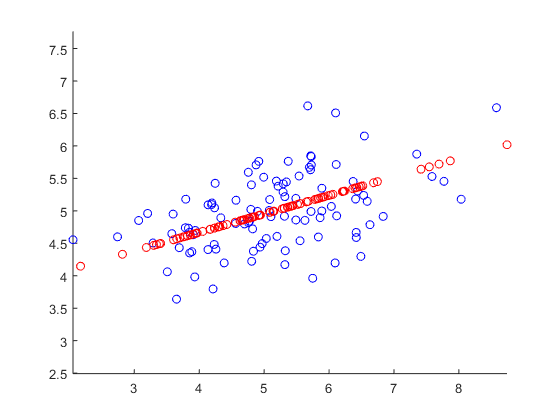
\includegraphics{task1.png}
\end{figure}

\item Součet čtverců kolmých vzdáleností bodů k nalezené přímce je
\begin{gather*}
\sum_{i=1}^{m} ||a_i-\tilde{a}_i||^2 = 24.2419
\end{gather*}

\item Hledaný vektor $x = (0.2740, -0.9617)$ je normálový vektor hledané přímky. Číslo $\alpha = -3.3931$ jsem dostal po dosazení bodu $y$ z hledané přímky a normálového vektoru $x$ do rovnice $y^Tx = \alpha$. Vektor $s = (-0.9617, -0.2740)$ je směrovým vektorem hledané přímky a bod $y_{0} = (-0.9296, 3.2633)$ se spočítá ze soustavy rovnic:
\begin{gather*}
y_0^Tx  = \alpha \\
y_0^Ts = 0
\end{gather*}

Kde první rovnice je obecná rovnice hledané přímky a druhá rovnice je obecná rovnice přímky kolmé na tu první a procházející počátkem, $y_0$ je tedy jejich průsečík.

\end{enumerate}
\section{Úloha 2: Komprese sekvence z motion capture}
\begin{enumerate}
\item Optimální hodnoty r:
\begin{center}
\begin{tabular}{|c|c|}
\hline
r & $\sum_{i=1}^{m} ||a_i-\tilde{a}_i||^2$\T\B \\
\hline
 1 & $4.616623 \cdot 10^8$ \\
 2 & $1.692542 \cdot 10^8$ \\
 5 & $1.0453 \cdot 10^7$ \\
 10 & $1.198151 \cdot 10^6$ \\
 15 & $2.562606 \cdot 10^5$ \\
\hline
\end{tabular}
\end{center}

\item Grafy
\begin{figure}[H]
	\centering
	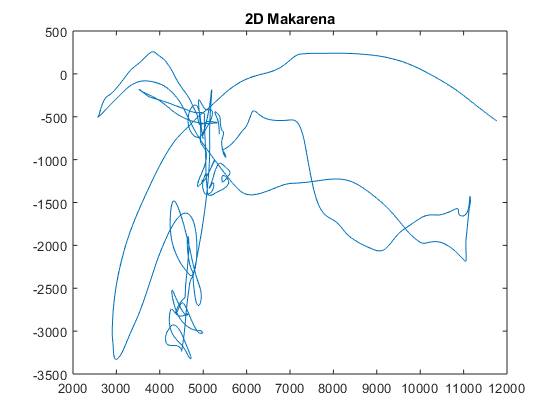
\includegraphics{makarena_2d.png}
\end{figure}
\noindent

\begin{figure}[H]
	\centering
	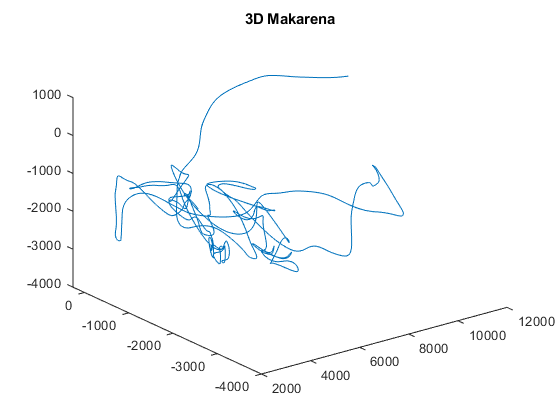
\includegraphics{makarena_3d.png}
\end{figure}
\noindent

\begin{figure}[H]
	\centering
	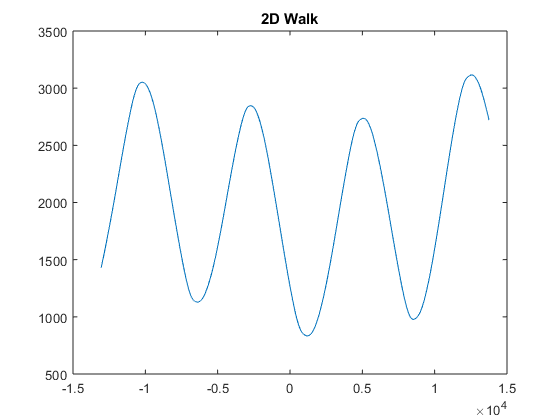
\includegraphics{walk_2d.png}
\end{figure}
\noindent

\begin{figure}[H]
	\centering
	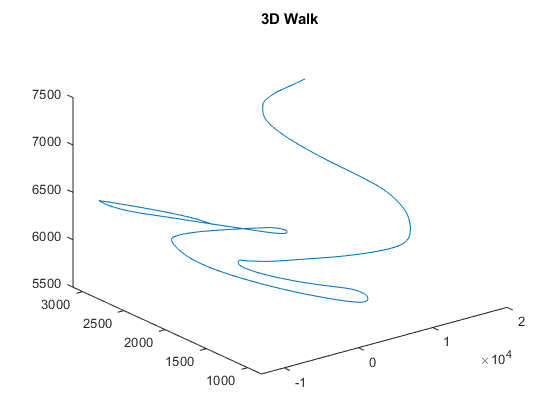
\includegraphics{walk_3d.png}
\end{figure}
\noindent

\item Minimální dimenze podprostoru je \b{1}. Všechny body v případě translačního pohybu se pohybují po rovnoběžných přímkách, stačí nám tedy znát jeden směrový vektor. Polohu všech bodů v kterémkoli okamžiku můžeme zjistit pak z rovnice $y_0+ts$, kde za $y_0$ postupně dosadíme počáteční body a $s$ je směrový vektor.

\item Hledaný vztah se dá vyjádřit následující rovností:
\begin{gather*}
\sum_{i=1}^{m} ||a_i-\tilde{a}_i||^2 = s_{r+1}^2 + \ldots + s_{n}^2
\end{gather*}
Kde $(s_{r+1},\ldots,s_{n})$ jsou vynulovaná singulární čísla.

\end{enumerate}

\end{document}